\documentclass[11pt, a4paper]{article}

% --- UNIVERSAL PREAMBLE BLOCK ---
\usepackage[a4paper, top=2.5cm, bottom=2.5cm, left=2cm, right=2cm]{geometry}
\usepackage{fontspec}
\usepackage{graphicx}

\usepackage[czech, bidi=basic, provide=*]{babel}

\babelprovide[import, onchar=ids fonts]{czech}
\babelprovide[import, onchar=ids fonts]{english}

% Set default/Latin font to Sans Serif in the main (rm) slot
\babelfont{rm}{Noto Sans}

% Add because main language is not English
\usepackage{enumitem}
\setlist[itemize]{label=-}
% --- END UNIVERSAL PREAMBLE BLOCK ---

\usepackage{booktabs}
\usepackage{tabularx}
\usepackage{hyperref}

\hypersetup{
    colorlinks=true,
    linkcolor=blue,
    filecolor=magenta,      
    urlcolor=cyan,
    pdftitle={Semestrální projekt - Rezervace},
}

\begin{document}

% --- TITULNÍ STRANA ---
\begin{titlepage}
    \centering
    \vspace*{4cm}
    
    {\Huge \textbf{Platforma pro krátkodobé pronájmy nemovitostí}}
    
    \vspace{1.5cm}
    {\Large Semestrální projekt -- Sub-systém: Rezervace}
    
    \vspace{3cm}
    
    \begin{flushleft}
        \large
        
        \textbf{Tým:} \\
        Matúš Budoš - BUD0081 \\
        Kristián Válek - VAL0556 \\
        Vojtěch Lisztwan - LIS0168 \\
    \end{flushleft}
    
    \vfill
    
    {\large \today}
\end{titlepage}

% --- OBSAH ---
\tableofcontents
\newpage

% --- OBSAH DOKUMENTU ---

\section{Důvod a okolnosti zavedení řešení}
Platforma vzniká z potřeby digitálně a efektivně propojit majitele volných nemovitostí s hosty, kteří hledají krátkodobé ubytování. Cílem je plně automatizovat, zjednodušit a zabezpečit celý proces pronájmu od prvotního vyhledání bytu, přes blokaci termínu, až po úspěšné zaplacení a následné hodnocení pobytu. Odstraněním manuálních kroků se snižuje chybovost a riziko překryvu rezervací.

\section{Slovní zadání, popis projektu od zákazníka}
\textit{Zákazník (investor) přichází s požadavkem na vývoj nové, moderní platformy pro zprostředkování krátkodobých pronájmů, která má konkurovat stávajícím řešením na trhu lepším uživatelským zážitkem a nižšími transakčními poplatky pro lokální trh.}

\vspace{0.3cm}
\noindent \textbf{Motivace a vize:} 
Cílem projektu je vytvořit ucelený informační systém fungující jako oboustranné tržiště (marketplace). Na jedné straně stojí pronajímatelé, kterým systém musí poskytnout jednoduché rozhraní pro evidenci majetku, správu dostupnosti a cenotvorbu. Na straně druhé jsou hosté, kteří vyžadují rychlý a intuitivní způsob, jak najít ubytování podle svých preferencí (lokalita, termín, kapacita).

\vspace{0.3cm}
\noindent \textbf{Klíčové procesy (Core Business):}
Absolutním jádrem platformy je spolehlivý rezervační engine. Zákazník striktně vyžaduje plnou automatizaci procesu -- od okamžiku, kdy host klikne na tlačítko "Rezervovat", se systém musí postarat o dočasné uzamčení termínu, aby nedošlo k tzv. overbookingu (dvojí rezervaci stejného termínu). Následně musí proběhnout hladké předání zákazníka na externí platební bránu a po úspěšné transakci automatické potvrzení rezervace oběma stranám via e-mail.

\vspace{0.3cm}
\noindent \textbf{Očekávaný výstup:}
Systém musí být nasaditelný v cloudovém prostředí (24/7), musí obsahovat administrátorský panel pro řešení sporů a moderaci obsahu. Velký důraz je kladen na modul hodnocení, který buduje důvěru v rámci komunity. Dostupnost termínů se nesmí ukládat staticky pro každý den, ale musí být počítána dynamicky na základě existujících blokací a platných rezervací, což zajistí vysokou konzistenci dat.

\section{Seznam modulů projektu a jejich významných atributů}
Systém se skládá ze 6 logických celků s definovanými datovými strukturami a unikátní identifikací.

\begin{enumerate}
    \item \textbf{Modul správy identit}
    \begin{itemize}
        \item \textit{Objekt Uživatel:} \texttt{id} (PK), \texttt{email} (unikátní), \texttt{password\_hash}, \texttt{jmeno}, \texttt{prijmeni}, \texttt{role} (Host / Pronajímatel / Administrátor).
    \end{itemize}
    
    \item \textbf{Modul správy nemovitostí}
    \begin{itemize}
        \item \textit{Objekt Nemovitost:} \texttt{id} (PK), \texttt{owner\_id} (FK), \texttt{nazev}, \texttt{popis}, \texttt{lokalita}, \texttt{max\_kapacita}, \texttt{standardni\_cena\_noc}.
        \item \textit{Objekt Fotografie:} \texttt{id} (PK), \texttt{property\_id} (FK), \texttt{cesta\_k\_souboru}.
        \item \textit{Objekt Blokace:} \texttt{id} (PK), \texttt{property\_id} (FK), \texttt{datum\_od}, \texttt{datum\_do}, \texttt{duvod}.
    \end{itemize}
    
    \item \textbf{Rezervační modul}
    \begin{itemize}
        \item \textit{Objekt Rezervace:} \texttt{id} (PK), \texttt{guest\_id} (FK), \texttt{property\_id} (FK), \texttt{datum\_zacatku}, \texttt{datum\_konce}, \texttt{celkova\_cena}, \texttt{stav} (Pending / Confirmed / Cancelled).
    \end{itemize}
    
    \item \textbf{Platební modul}
    \begin{itemize}
        \item \textit{Objekt Platba:} \texttt{id} (PK), \texttt{reservation\_id} (FK), \texttt{transakce\_brany\_id} (unikátní), \texttt{castka}, \texttt{stav\_platby}.
    \end{itemize}
    
    \item \textbf{Modul hodnocení}
    \begin{itemize}
        \item \textit{Objekt Recenze:} \texttt{id} (PK), \texttt{reservation\_id} (FK), \texttt{autor\_id} (FK), \texttt{text}, \texttt{hvezdicky} (1-5).
    \end{itemize}
    
    \item \textbf{Administrátorský panel}
    \begin{itemize}
        \item \textit{Objekt Log:} \texttt{id} (PK), \texttt{akce}, \texttt{casove\_razitko}, \texttt{admin\_id}.
    \end{itemize}
\end{enumerate}

\section{Systémové požadavky FURPS}

\subsection*{a. Funkčnost (Functionality – F)}
\begin{itemize}
    \item \textbf{Správa identit:} Systém musí umožňovat bezpečné zakládání uživatelských účtů s rozdělením rolí a autentizaci (přihlašování).
    \item \textbf{Správa nabídek:} Pronajímatelé musí mít možnost provádět CRUD operace (Create, Read, Update, Delete) nad svými nemovitostmi, nahrávat fotografie a definovat výjimky v kalendáři (např. blokace z důvodu malování).
    \item \textbf{Rezervační proces:} Systém musí umět dynamicky vyhledávat volné kapacity na základě zadaných parametrů, dočasně uzamknout zvolený termín pro konkrétního uživatele a spravovat životní cyklus rezervace.
    \item \textbf{Platební integrace:} Plná integrace na externí platební bránu s automatickým zpracováním HTTP webhooků pro potvrzení transakcí.
\end{itemize}

\subsection*{b. Vhodnost k použití (Usability – U)}
\begin{itemize}
    \item \textbf{Responzivní design (Mobile-first):} Klientská část aplikace (vyhledávání, rezervace) musí být plně optimalizována pro mobilní telefony, odkud se očekává většina provozu.
    \item \textbf{Transparentnost cen:} Host musí před započetím platby vidět jasný a detailní rozpis ceny (počet nocí $\times$ cena za noc + případné poplatky).
    \item \textbf{Intuitivní kalendář:} Pronajímatelům musí být k dispozici vizuální kalendář pro snadnou správu dostupnosti a rychlý přehled o obsazenosti.
    \item \textbf{Jasná zpětná vazba:} Systém musí uživateli poskytovat srozumitelné chybové hlášky, zejména v případě selhání platby nebo při obsazení termínu jiným uživatelem.
\end{itemize}

\subsection*{c. Spolehlivost (Reliability – R)}
\begin{itemize}
    \item \textbf{Integrita dat (Zamezení Overbookingu):} Rezervační logika musí využívat ACID transakce na úrovni databáze (např. pesimistické zamykání řádků), aby se v případě souběhu požadavků nikdy nerezervoval stejný byt dvěma lidem.
    \item \textbf{Automatická obnova (Self-healing):} Nedokončené nebo nezaplacené rezervace (tzv. uvízlé transakce) musí systém prostřednictvím plánovaných úloh (CRON) po určité době sám stornovat a termíny uvolnit.
    \item \textbf{Bezpečnost dat (GDPR):} Osobní údaje uživatelů a detaily o platbách musí být chráněny proti neoprávněnému přístupu (šifrování hesel, HTTPS komunikace).
\end{itemize}

\subsection*{d. Výkon (Performance – P)}
\begin{itemize}
    \item \textbf{Rychlost vyhledávání:} Odezva systému při složitém dotazování (filtrace dle parametrů spojená s dynamickým přepočtem kalendáře) nesmí přesáhnout 2 sekundy.
    \item \textbf{Rychlost transakcí:} Dočasné uzamčení termínu v databázi při kliknutí na "Rezervovat" musí proběhnout v řádu milisekund, aby se minimalizovalo okno pro race-condition.
    \item \textbf{Škálovatelnost:} Systém musí být schopen zvládnout nárazové špičky návštěvnosti (např. vyhledávání chat na horách před Silvestrem nebo prázdninami).
\end{itemize}

\subsection*{e. Schopnost údržby (Supportability – S)}
\begin{itemize}
    \item \textbf{Modulární architektura:} Logika aplikace musí být striktně oddělena do 6 popsaných modulů. Případná chyba v modulu hodnocení nesmí shodit proces rezervace.
    \item \textbf{Rozšiřitelnost API:} Komunikace s externími poskytovateli (platební brána, e-mail server) musí být navržena přes rozhraní (Interfaces/Adapters). Pokud se v budoucnu změní poskytovatel (např. přechod ze Stripe na GoPay), postačí napsat nový adaptér, bez zásahu do core byznys logiky.
    \item \textbf{Auditovatelnost:} Všechny kritické systémové operace (tvorba rezervace, platba, zrušení, ban uživatele) musí být trvale zaznamenávány v systémovém logu pro případné zpětné trasování chyb či sporů.
\end{itemize}

\section{Kritické situace}

\begin{itemize}
    \item \textbf{Systémové (Výpadek konektivity externí služby):} Host zaplatí, peníze se strhnou z jeho bankovního účtu, ale dojde k výpadku sítě a naše platforma nedostane webhook od platební brány o úspěšnosti. Systém si tak myslí, že je rezervace nezaplacena.
    \item \textbf{Aplikační (Souběh transakcí - Race Condition):} Dva různí hosté mají otevřený stejný detail nemovitosti na velmi žádaný termín (např. Silvestr). Oba kliknou na tlačítko "Rezervovat" ve stejnou vteřinu. Pokud by nedošlo k ošetření zámkem, systém by mohl povolit půjčit stejný byt dvěma lidem na stejný termín, což nesmí nastat.
\end{itemize}

\section{Hranice systému}

\begin{itemize}
    \item \textbf{Ideální scénář:} Pronajímatel vloží plnohodnotně vyplněnou nabídku. Host aplikuje filtry, ihned najde volnou nemovitost, provede rezervaci, okamžitě zaplatí platební kartou. Systém stav změní na "Potvrzeno", propíše termín do kalendáře a pošle e-maily. Pobyt bez problémů proběhne.
    
    \item \textbf{Hraničně řešitelný scénář:} Host si zarezervuje byt, čímž termín na 15 minut zablokuje, ale v průběhu platby mu selže prohlížeč nebo záměrně okno zavře a nezaplatí. Systém na pozadí pomocí vlastních naplánovaných úloh (CRON) identifikuje nedokončenou rezervaci po vypršení limitu, automaticky ji stornuje a uvolní termín dalším uživatelům bez zásahu administrátora.
    
    \item \textbf{Situace, které systém nezvládne vyřešit:} Host přijede na místo ubytování a úmyslně fyzicky zničí vybavení bytu. Náš software sice umožní pronajímateli zanechat špatné hodnocení a případně může administrátor zablokovat uživatelský účet hosta, ale fyzické vymáhání škody, pojišťovací řízení či samotná oprava leží kompletně mimo hranice tohoto informačního systému.
\end{itemize}

\section{Kontext prostředí}
Platforma funguje jako webová aplikace v cloudovém prostředí. Běží 24/7 a slouží jako prostředník (marketplace). Systém negeneruje vlastní obsah, veškerá nabídka vzniká na straně pronajímatelů a poptávka na straně návštěvníků. Operuje v prostředí internetu s nutností zabezpečené komunikace (HTTPS) a striktním dodržováním nakládání s osobními údaji (GDPR).

\section{Charakteristika aktérů a prostředí}

\subsection*{a. Aktéři, uživatelé, role}
\begin{itemize}
    \item \textbf{Host (Návštěvník):} Vyhledává ubytování, provádí rezervace a platby, uděluje hodnocení.
    \item \textbf{Pronajímatel (Majitel nemovitosti):} Zakládá profily nemovitostí, nahrává fotky, definuje ceny a kalendář blokací.
    \item \textbf{Administrátor:} Řeší spory, má právo rušit účty a moderovat nabídky, kontroluje systémové logy.
    \item \textbf{Systém (Časovač/CRON):} Autonomní vnitřní aktér spouštějící periodické čistící procesy (např. rušení nezaplacených rezervací).
\end{itemize}

\subsection*{b. Externí systémy}
\begin{itemize}
    \item \textbf{Platební brána:} Zpracovává platby z karet a vrací systému status transakce.
    \item \textbf{E-mailový server (SMTP/API):} Fyzicky doručuje notifikace do schránek uživatelů.
    \item \textbf{Mapové služby:} Validují GPS souřadnice a vizualizují lokality ubytování.
\end{itemize}

\section{Use case diagramy}

\subsection{Modul správy uživatelů}

% Zde kolega [Jméno 2] vloží svůj popis k Use case diagramu a nahradí obrázek
\begin{figure}[htbp]
  \centering
  \framebox{\parbox{0.8\textwidth}{\centering
    \vspace{2cm}
    \textbf{Zde bude Use Case diagram pro správu uživatelů} \\
    \vspace{2cm}
  }}
  \caption{Use Case diagram pro modul správy uživatelů.}
\end{figure}

\subsection{Modul správy nemovitostí}

\begin{figure}[htbp]
  \centering
  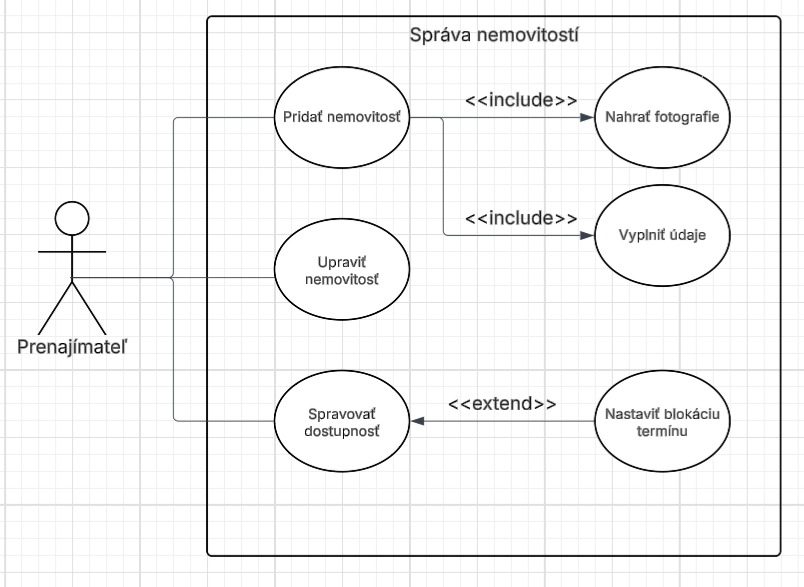
\includegraphics[width=0.95\textwidth]{usecaseNemovitosti.png}
  \caption{Use Case diagram pre správu nemovitostí.}
  \label{fig:uc_diagram_rezervace}
\end{figure}

\subsection{Rezervační modul}

Diagram pokrývá logický celek rezervací. Zahrnuje komunikaci mezi Hostem, Časovačem, Platební bránou a pěti moduly platformy.

\begin{itemize}
    \item \textbf{Aktéři:} Host (Primární), Platební brána (Sekundární), Systém (Časovač - Sekundární).
    \item \textbf{Moduly zapojené do UC:} Rezervační (Core pro tuto část), Platební, Správa nemovitostí, Identit, Komunikační.
    \item \textbf{Popis vazeb:}
    \begin{enumerate}
        \item Host iniciuje Use Case \textbf{"Vytvořit rezervaci"}.
        \item "Vytvořit rezervaci" má \texttt{\textless\textless include\textgreater\textgreater} na \textbf{"Ověřit dostupnost termínu"} a \textbf{"Ověřit identitu hosta"}.
        \item Na "Vytvořit rezervaci" navazuje přes \texttt{\textless\textless extend\textgreater\textgreater} (podmíněně, pokud se vytvoří) Use Case \textbf{"Provést platbu"}.
        \item U "Provést platbu" participuje externí aktér \textbf{Platební brána}.
        \item "Provést platbu" má \texttt{\textless\textless include\textgreater\textgreater} na \textbf{"Odeslat potvrzovací e-mail"}.
        \item Systémový časovač iniciuje UC \textbf{"Stornovat expirovanou rezervaci"}.
        \item Host iniciuje UC \textbf{"Zrušit zaplacenou rezervaci"}, s vazbou \texttt{\textless\textless include\textgreater\textgreater} na \textbf{"Provést refundaci"}.
    \end{enumerate}
\end{itemize}

\begin{figure}[htbp]
  \centering
  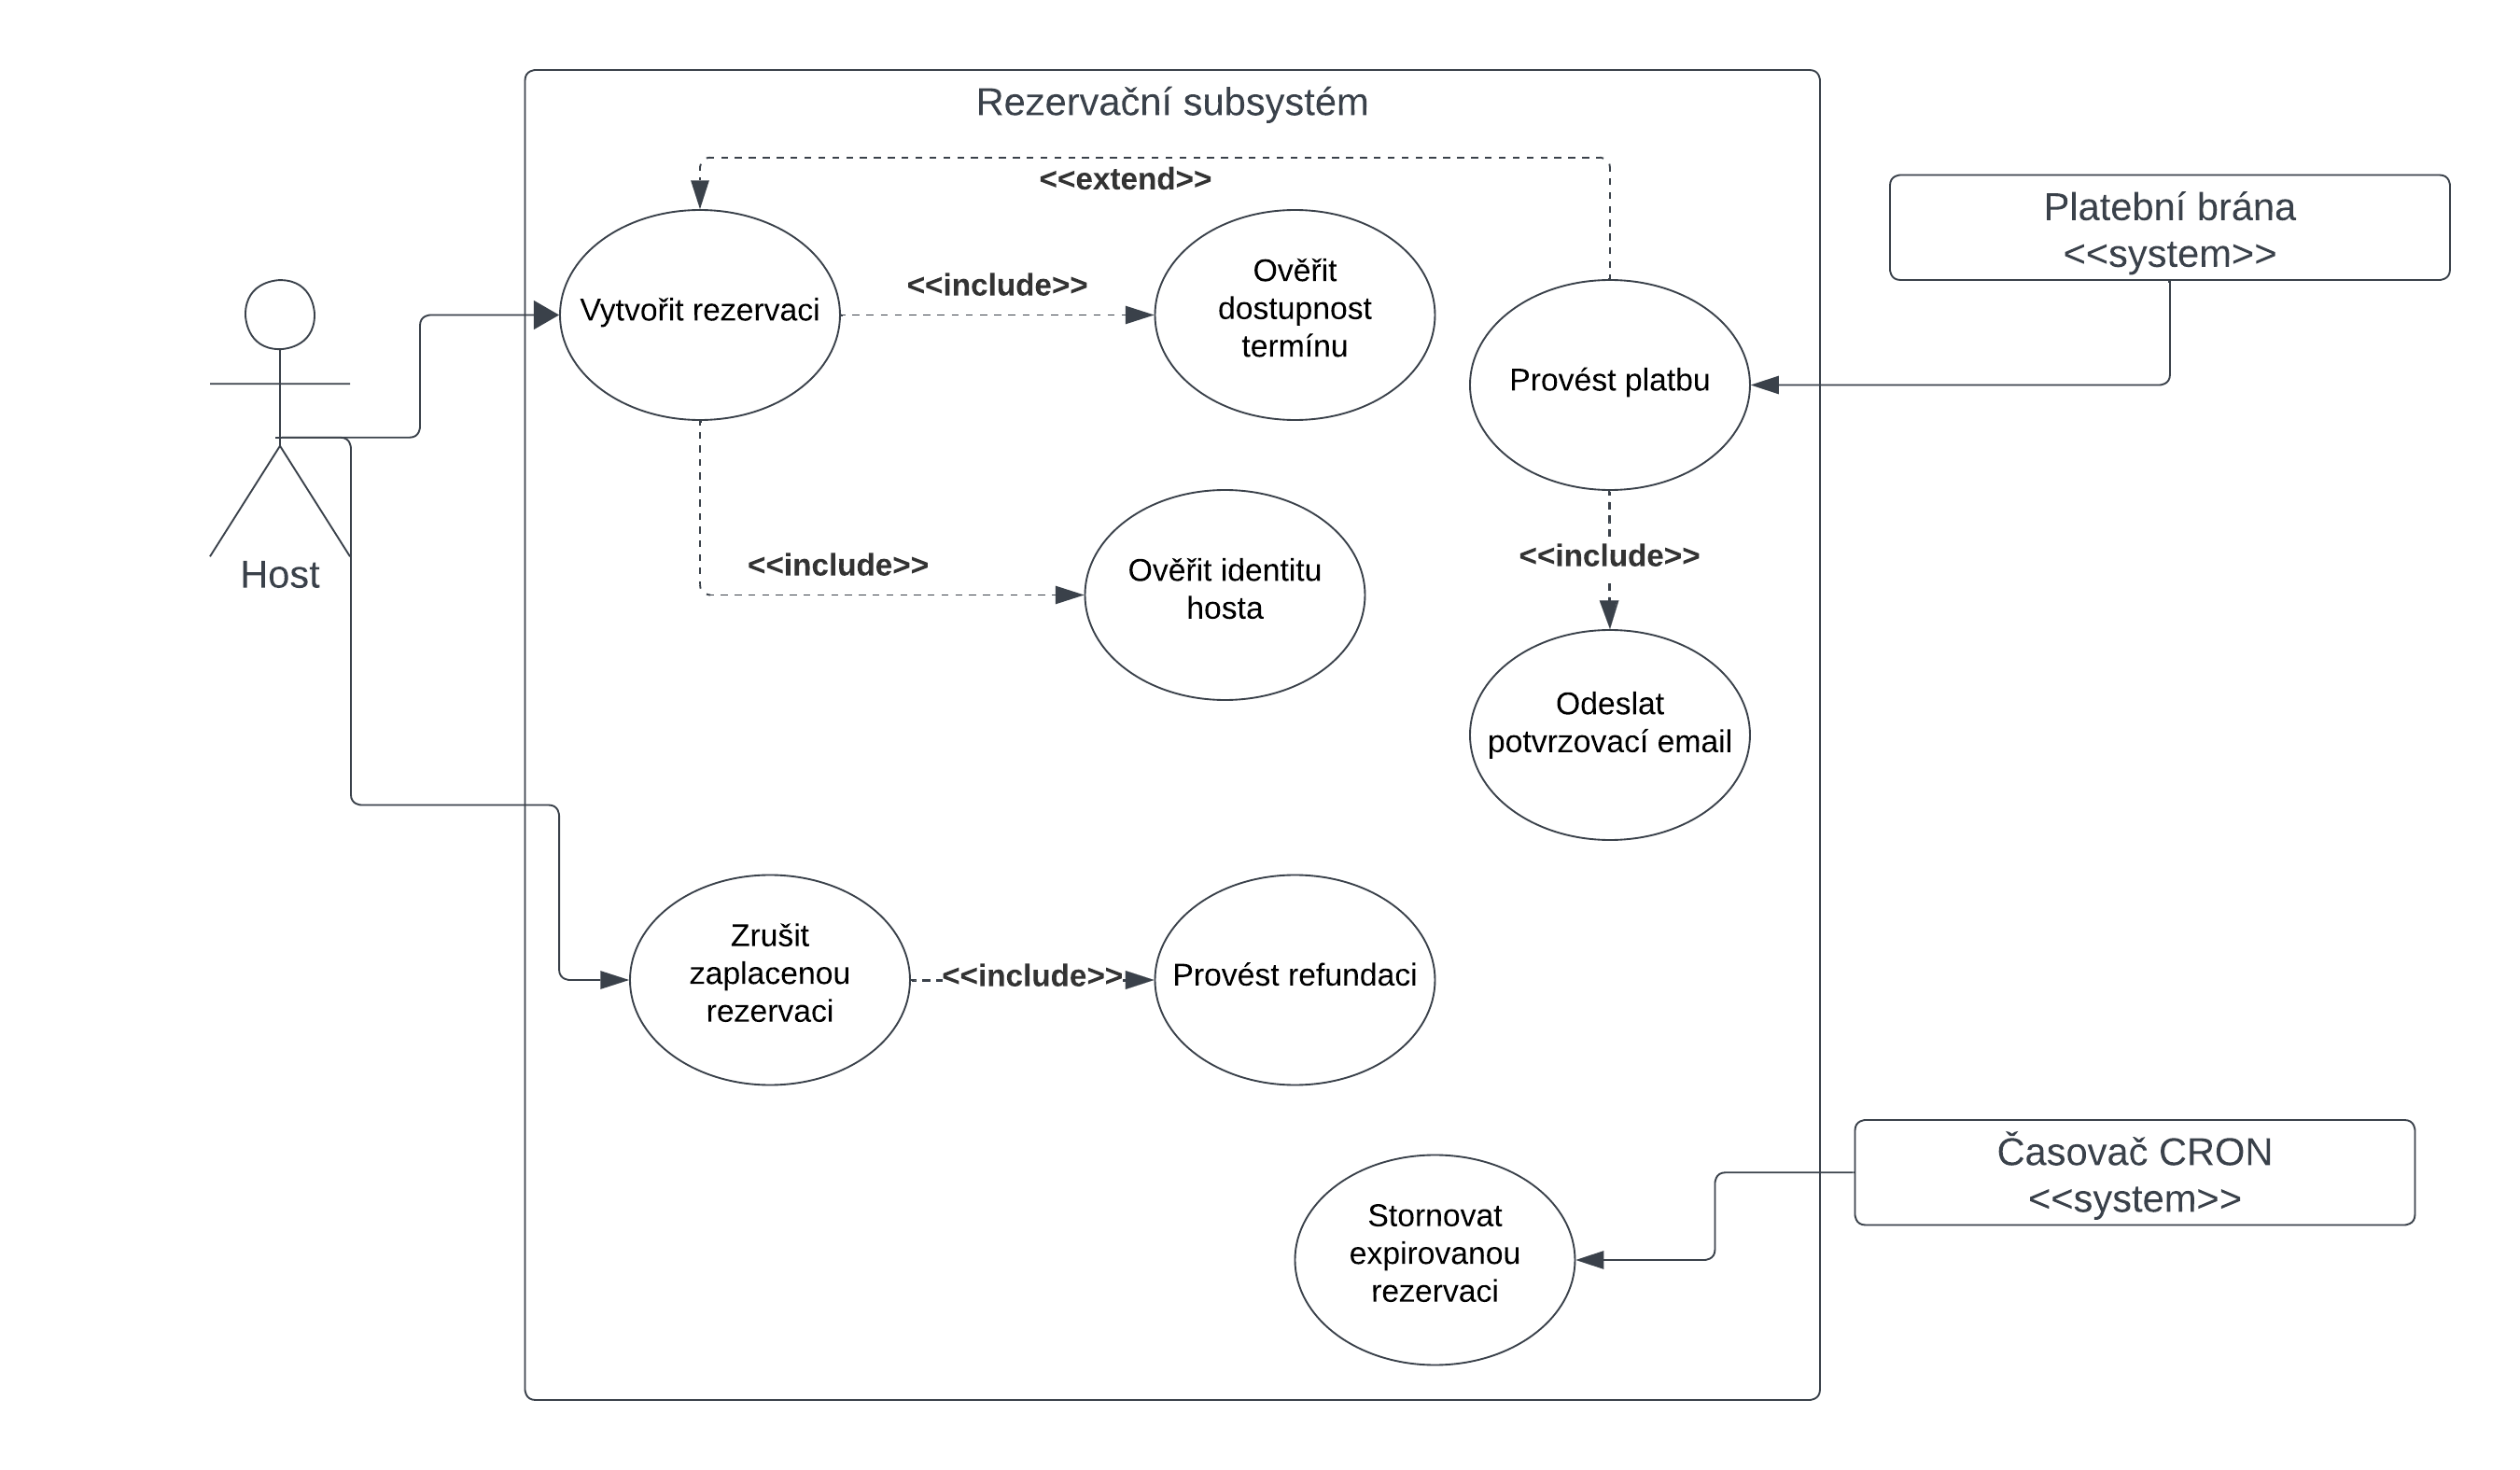
\includegraphics[width=0.95\textwidth]{usecase_rezervace.png}
  \caption{Use Case diagram pro rezervační sub-systém.}
  \label{fig:uc_diagram_rezervace}
\end{figure}

\newpage
\section{Scénáře (Konkrétní implementace Use Case)}

\subsection{Modul správy uživatelů}

% Zde kolega [Jméno 2] rozepíše své 3 scénáře
\subsubsection{Scénář 1: [Název prvního scénáře]}
\textit{[Kolega doplní kontext, aktéry, vstupní podmínky a kroky scénáře...]}

\subsubsection{Scénář 2: [Název druhého scénáře]}
\textit{[Kolega doplní...]}

\subsubsection{Scénář 3: [Název třetího scénáře]}
\textit{[Kolega doplní...]}


\vspace{1cm}
\subsection{Modul správy nemovitostí}

% Zde kolega [Jméno 1] rozepíše své 3 scénáře
\subsubsection{Scénář 1: [Název prvního scénáře]}
\textit{[Kolega doplní kontext, aktéry, vstupní podmínky a kroky scénáře...]}

\subsubsection{Scénář 2: [Název druhého scénáře]}
\textit{[Kolega doplní...]}

\subsubsection{Scénář 3: [Název třetího scénáře]}
\textit{[Kolega doplní...]}


\newpage
\subsection{Rezervační modul}

\subsubsection{Scénář 1: Vytvoření rezervace a platba}
\begin{itemize}[leftmargin=*]
    \item \textbf{Název:} Zpracování rezervace a úhrady ubytování.
    \item \textbf{Kontext:} Host si vybral termín, klikl na tlačítko "Rezervovat". Probíhá uzamčení termínu a převod peněz.
    \item \textbf{Level zanoření Use Case:} Uživatelský cíl (Hlavní proces).
    \item \textbf{Aktéři:} Host, Platební brána (externí systém).
    \item \textbf{Stakeholdeři a zájmové osoby:} Pronajímatel (očekává zisk a informaci o obsazení bytu).
    \item \textbf{Vstupní podmínky:} Host je autentizován, požadovaný termín vybraného bytu je aktuálně volný.
    \item \textbf{Výstupní podmínky:} Systém eviduje rezervaci ve stavu \textit{Confirmed}, na platbě je stav \textit{Success}, termín je závazně blokován v kalendáři nemovitosti.
    \item \textbf{Minimální výstup:} Vytvoření dočasného záznamu v databázi se statusem \textit{Pending} (při nedokončení).
    \item \textbf{Ideální výstup:} Úspěšná platba, propis potvrzení a odeslání oboustranného e-mailového upozornění (voucheru).
\end{itemize}

\noindent \textbf{Hlavní scénář:}
\begin{enumerate}
    \item \textbf{Host} zadá data a potvrdí parametry rezervace.
    \item \textbf{Systém} dotáže modul správy nemovitostí a naposledy ověří dostupnost.
    \item \textbf{Systém} vytvoří záznam rezervace se stavem \textit{Pending} a aplikuje dočasný zámek termínu.
    \item \textbf{Systém} přesměruje relaci Hosta na \textit{Platební bránu}.
    \item \textbf{Host} (v externím rozhraní) vyplní údaje a potvrzuje platbu.
    \item \textbf{Platební brána} zpracuje transakci a odešle do Systému webhook o výsledku.
    \item \textbf{Rozhodování:} Zda je webhook úspěšný. (V tomto kroku ano).
    \item \textbf{Systém} na základě kladného výsledku mění stav rezervace na \textit{Confirmed} a zámek na trvalý.
    \item \textbf{Systém} volá e-mailový modul pro odeslání dokladů.
\end{enumerate}

\noindent \textbf{Rozšíření:}
\begin{itemize}
    \item 2a. Termín byl obsazen někým jiným: Systém přeruší proces a vypíše chybovou zprávu. Konec případu užití.
    \item 6a. Karta je zamítnuta: Platební brána vrací chybový kód. Cyklus se vrací do bodu 5 a Systém vyzve Hosta k použití jiné karty, dokud nevyprší časový limit rezervace.
\end{itemize}

\vspace{0.5cm}
\subsubsection{Scénář 2: Automatické storno rezervace při nezaplacení}
\begin{itemize}[leftmargin=*]
    \item \textbf{Název:} Uvolnění termínu při selhání platby (Timeout).
    \item \textbf{Kontext:} Host vytvořil návrh rezervace, ale nedokončil platbu v určeném časovém okně (např. 15 minut).
    \item \textbf{Level zanoření Use Case:} Systémový cíl (Sub-funkce na pozadí).
    \item \textbf{Aktéři:} Systém (Časovač/CRON).
    \item \textbf{Stakeholdeři a zájmové osoby:} Pronajímatel (potřebuje mít byt přístupný pro jiné návštěvníky).
    \item \textbf{Vstupní podmínky:} Existuje rezervace ve stavu \textit{Pending}, u které uplynula povolená doba pro platbu.
    \item \textbf{Výstupní podmínky:} Rezervace má stav \textit{Cancelled} a dočasný zámek kalendáře je odstraněn.
    \item \textbf{Minimální výstup:} Uvolnění blokace nad nemovitostí.
    \item \textbf{Ideální výstup:} Uvolnění blokace a označení rezervace korektním stavovým kódem s případnou zprávou do logu.
\end{itemize}

\noindent \textbf{Hlavní scénář:}
\begin{enumerate}
    \item \textbf{Cyklus:} \textbf{Systém} (Časovač) se aktivuje každou 1 minutu.
    \item \textbf{Systém} prohledává databázi rezervací.
    \item \textbf{Rozhodování:} Nalezne-li záznamy \textit{Pending} starší než 15 min, pokračuje bodem 4. Jinak čeká na další cyklus.
    \item \textbf{Systém} se API dotazem ujistí u platební brány, zda nevisí nedokončená transakce.
    \item \textbf{Systém} změní stav u daného záznamu na \textit{Cancelled}.
    \item \textbf{Systém} uvolní všechny související datumové zámky.
    \item \textbf{Systém} odešle informační e-mail Hostovi o expiraci.
\end{enumerate}

\noindent \textbf{Rozšíření:}
\begin{itemize}
    \item 4a. API platební brány oznámí, že platba před okamžikem úspěšně prošla, ale nedošel webhook: Systém přeskočí zrušení, doplní platbu a změní stav rezervace na \textit{Confirmed}.
\end{itemize}

\vspace{0.5cm}
\subsubsection{Scénář 3: Zrušení zaplacené rezervace hostem}
\begin{itemize}[leftmargin=*]
    \item \textbf{Název:} Storno potvrzené rezervace se žádostí o refundaci.
    \item \textbf{Kontext:} Host má zaplacený pobyt v budoucnosti, ale klikne na "Zrušit rezervaci".
    \item \textbf{Level zanoření Use Case:} Uživatelský cíl.
    \item \textbf{Aktéři:} Host.
    \item \textbf{Stakeholdeři a zájmové osoby:} Pronajímatel (dozví se o zrušení pobytu).
    \item \textbf{Vstupní podmínky:} Host je přihlášen a eviduje u sebe rezervaci ve stavu \textit{Confirmed} s počátkem pobytu v budoucnosti.
    \item \textbf{Výstupní podmínky:} Rezervace je stornována (\textit{Cancelled}), prostředky se na pokyn systému vrací (refundují) a termín je opět volný.
    \item \textbf{Minimální výstup:} Změna stavu v databázi platformy a uvolnění kalendáře.
    \item \textbf{Ideální výstup:} Výpočet případného storno poplatku, úspěšné zadání refundace platební bráně a vyrozumění obou stran.
\end{itemize}

\noindent \textbf{Hlavní scénář:}
\begin{enumerate}
    \item \textbf{Host} vybere konkrétní rezervaci a vyvolá akci pro zrušení.
    \item \textbf{Systém} zkontroluje aktuální datum vůči počátku pobytu.
    \item \textbf{Systém} na základě časového odstupu vypočítá výši refundace.
    \item \textbf{Systém} zobrazí Hostovi rekapitulaci vratky.
    \item \textbf{Host} provede finální potvrzení storna.
    \item \textbf{Systém} ukládá stav \textit{Cancelled} k rezervaci.
    \item \textbf{Rozhodování:} Pokud je částka vratky větší než nula, pokračuje bodem 8.
    \item \textbf{Systém} odesílá požadavek na refundaci \textit{Platební bráně}.
    \item \textbf{Systém} likviduje zámek termínu.
    \item \textbf{Systém} notifikuje Hosta a Pronajímatele.
\end{enumerate}

\noindent \textbf{Rozšíření:}
\begin{itemize}
    \item 7a. Vratka je rovna nule (např. rušení pouhý den předem bez nároku na vrácení peněz): Krok 8 se přeskočí a termín se i tak uvolní (krok 9).
\end{itemize}

\newpage
\section{Popis změn v dokumentu}

% Prázdná tabulka verzí využívající profesionální booktabs
\begin{table}[htbp]
    \centering
    \renewcommand{\arraystretch}{1.3}
    \begin{tabular}{@{}c p{12cm}@{}}
        \toprule
        \textbf{Verze} & \textbf{Popis změn} \\
        \midrule
        % Zde můžete v budoucnu doplňovat jednotlivé verze
        & \\
        \bottomrule
    \end{tabular}
    \caption{Historie verzí dokumentu}
    \label{tab:verzovani}
\end{table}

\end{document}